\clearpage
\section{Data control region plots}
\label{sec:data-control-region-plots}

MC simulation is used in a number of ways in the analysis, including to train the \glspl{bdt} and to gain understanding of the composition of the background, and to test the logic of the background methods (closure tests). It is therefore useful to compare distributions of key observables in data and MC to verify that the simulation does not significantly diverge from the data. To avoid unblinding the data in sensitive regions, the figures show various CRs known to be devoid of signal. 

A useful validation \gls{cr} is the region obtained by selecting events with an event-based classifier score less than 0. In the following study, this region is examined for the dimuon category. A focus is made on the Phase 1 data set because it is affected by various data quality issues that are further addressed in Section~\ref{sec:data-quality}. The comparison is shown in Figure~\ref{fig:data-control-plots-dimuon-phase1}. Generally good agreement between data and simulation can be observed in the ratio panels.


\begin{figure}[!htb]
\centering
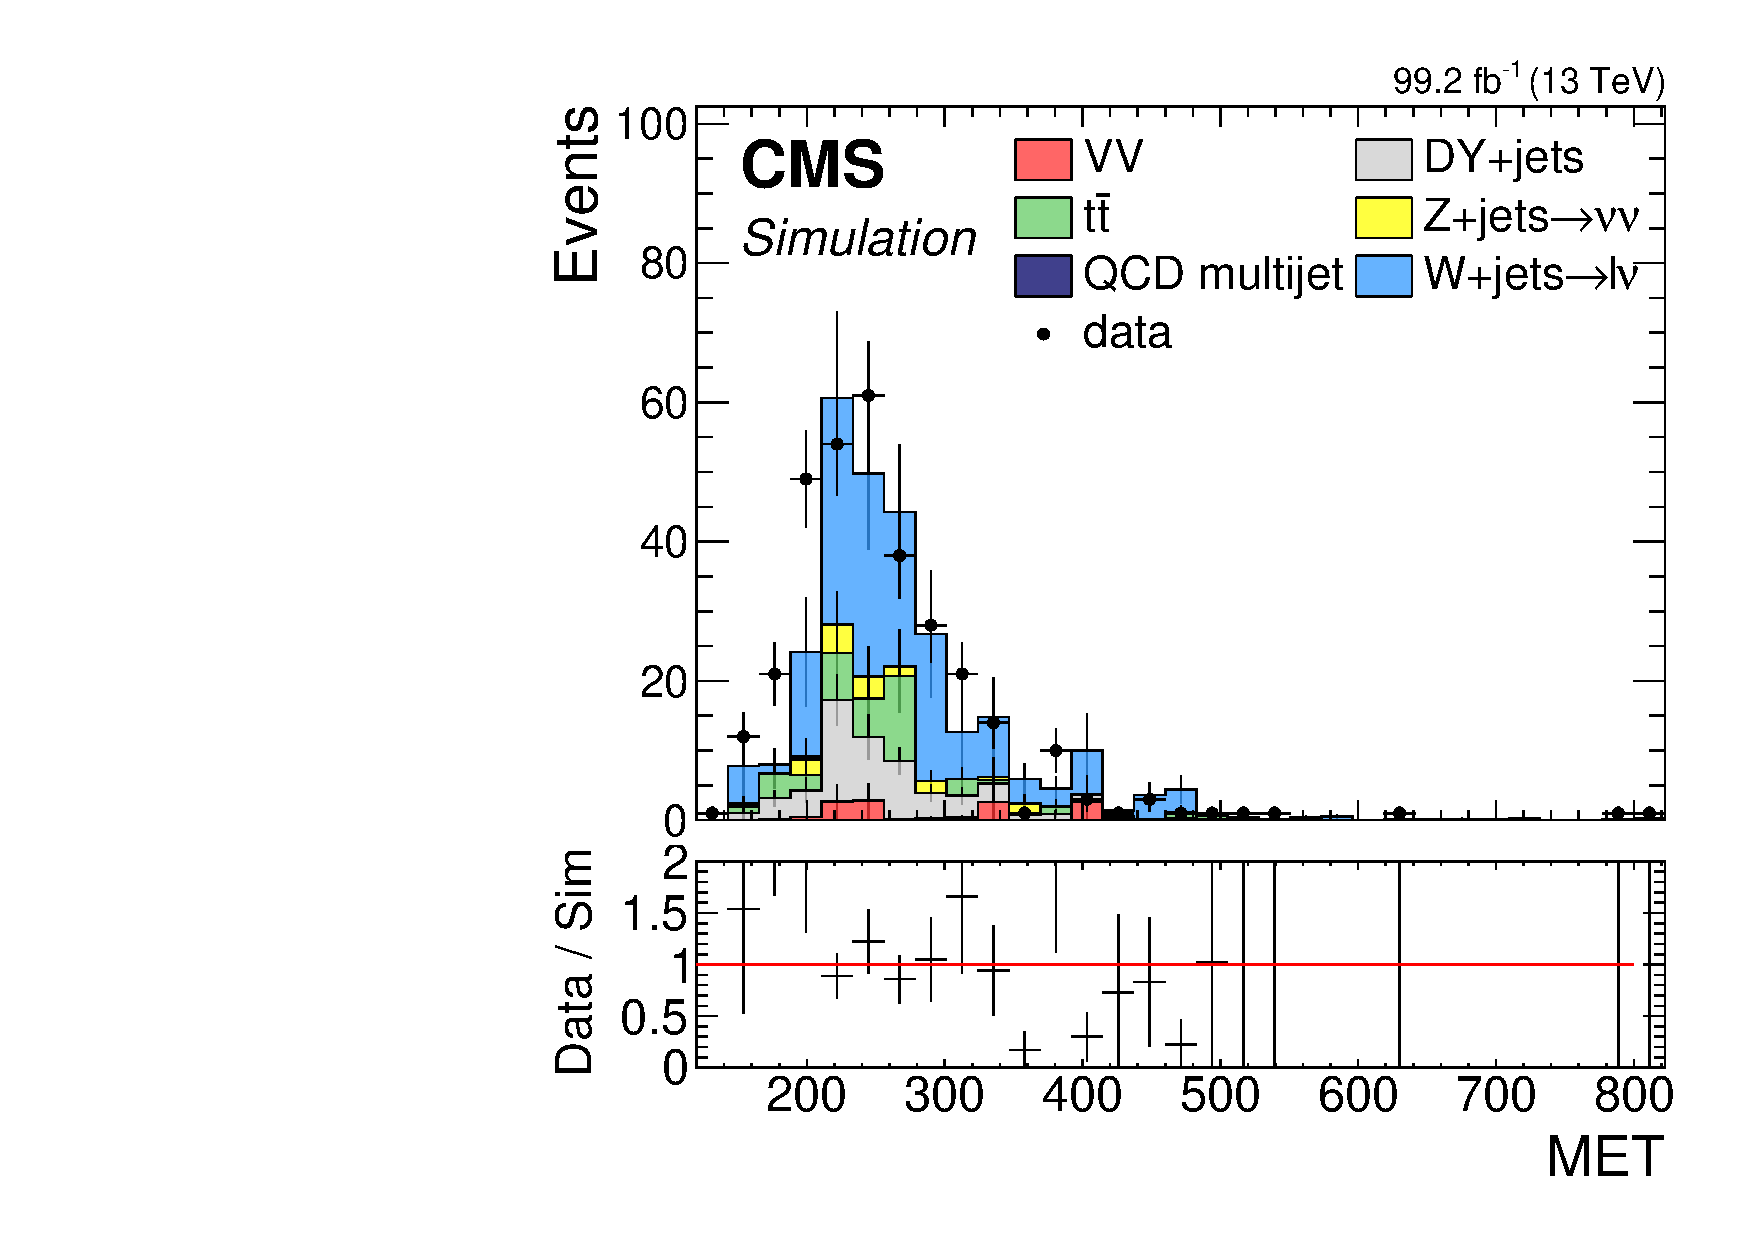
\includegraphics[width=0.48\linewidth]{plots/dilepton_muons_data_control_region_phase1/none_MET.pdf} \,
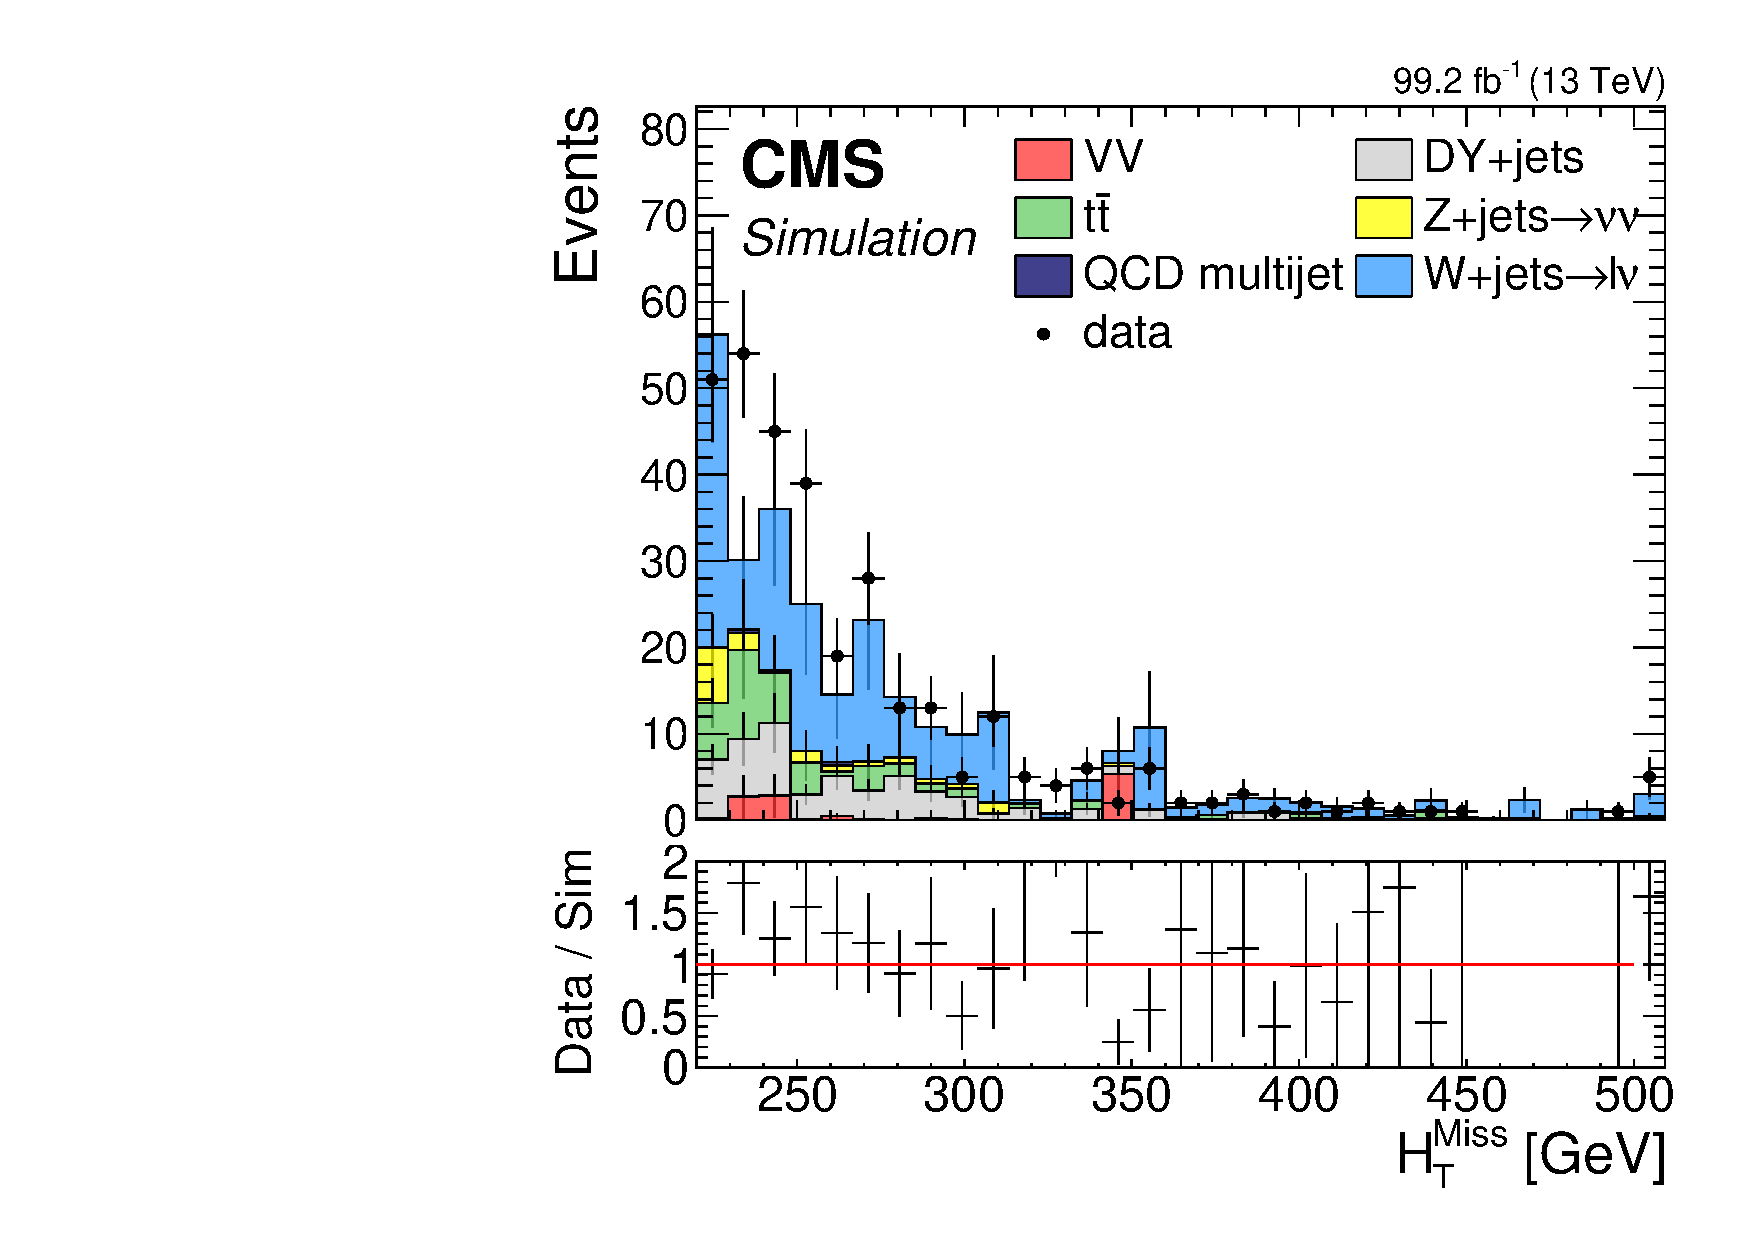
\includegraphics[width=0.48\linewidth]{plots/dilepton_muons_data_control_region_phase1/none_MHT.pdf} \\

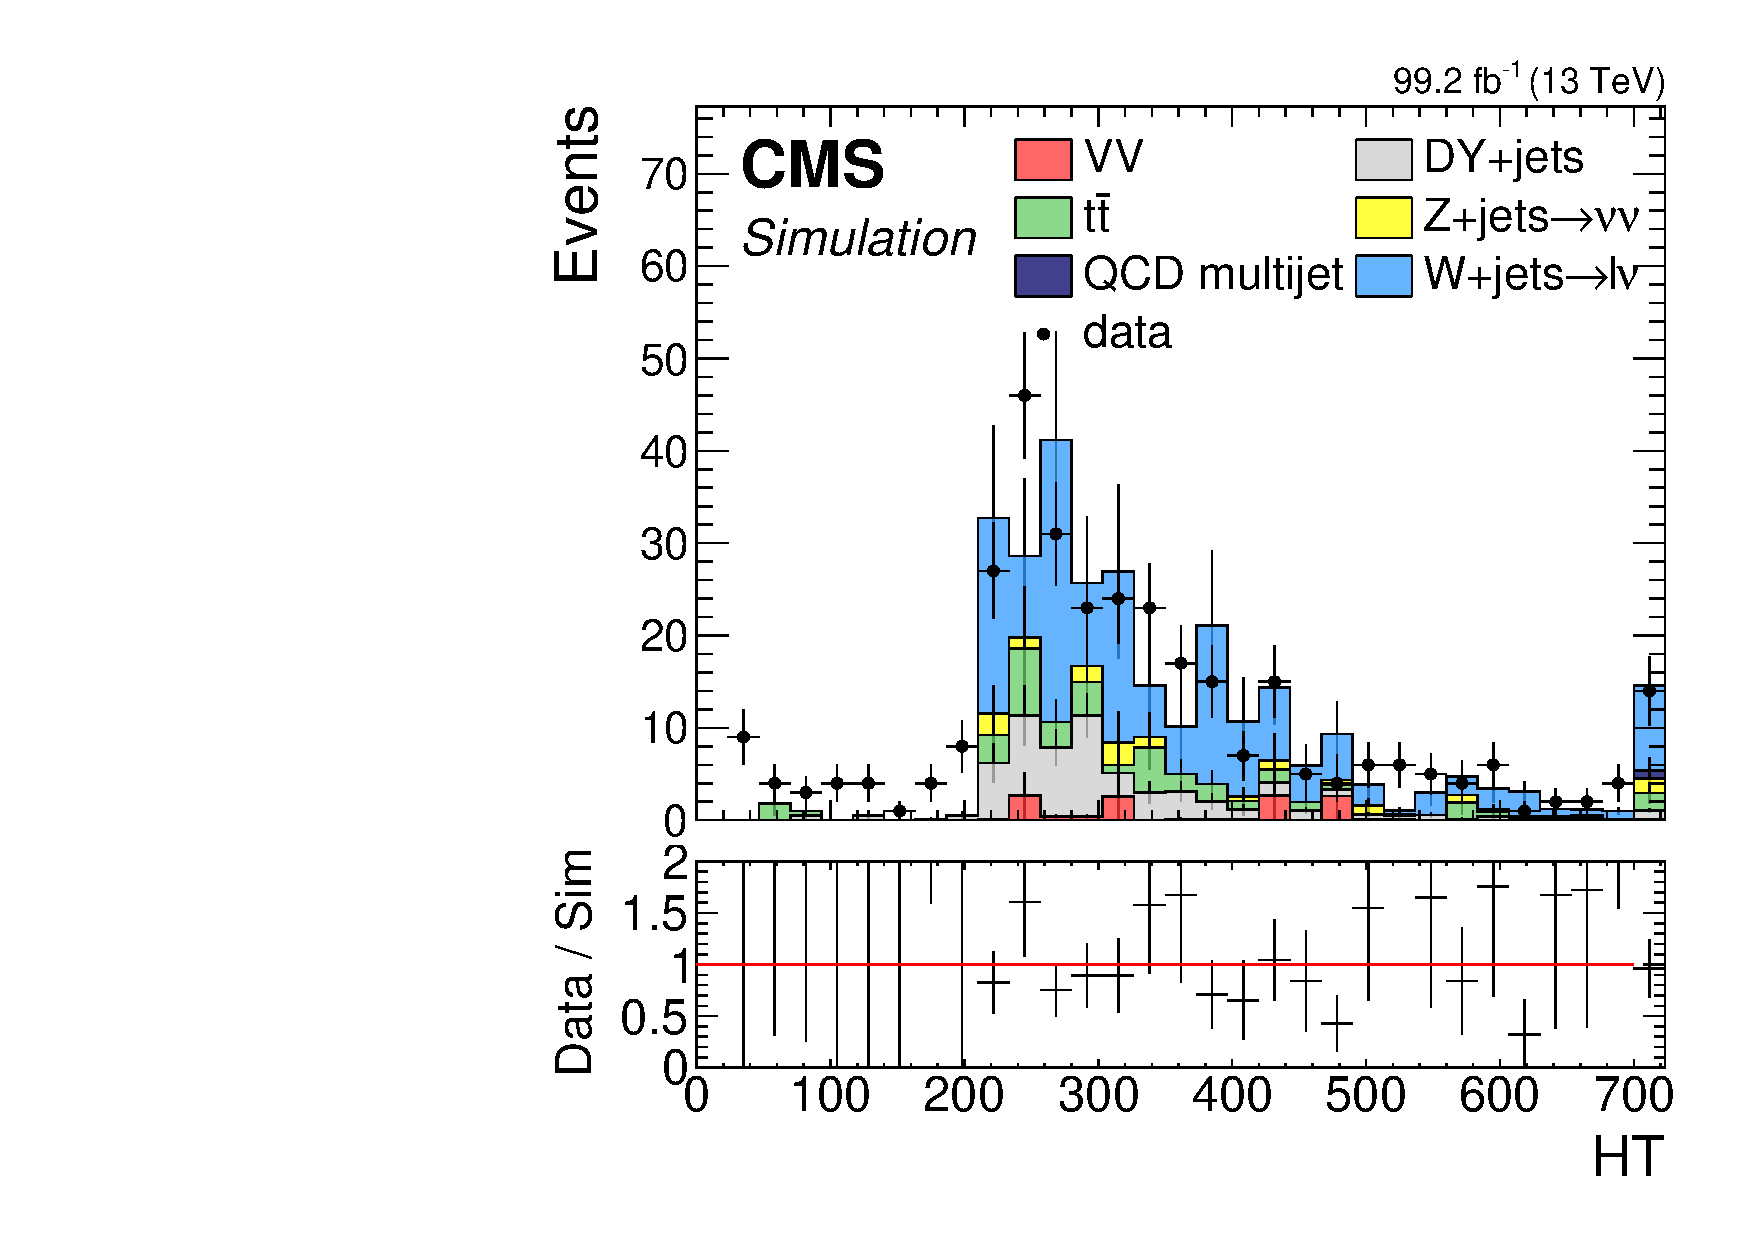
\includegraphics[width=0.48\linewidth]{plots/dilepton_muons_data_control_region_phase1/none_HT.pdf} \,
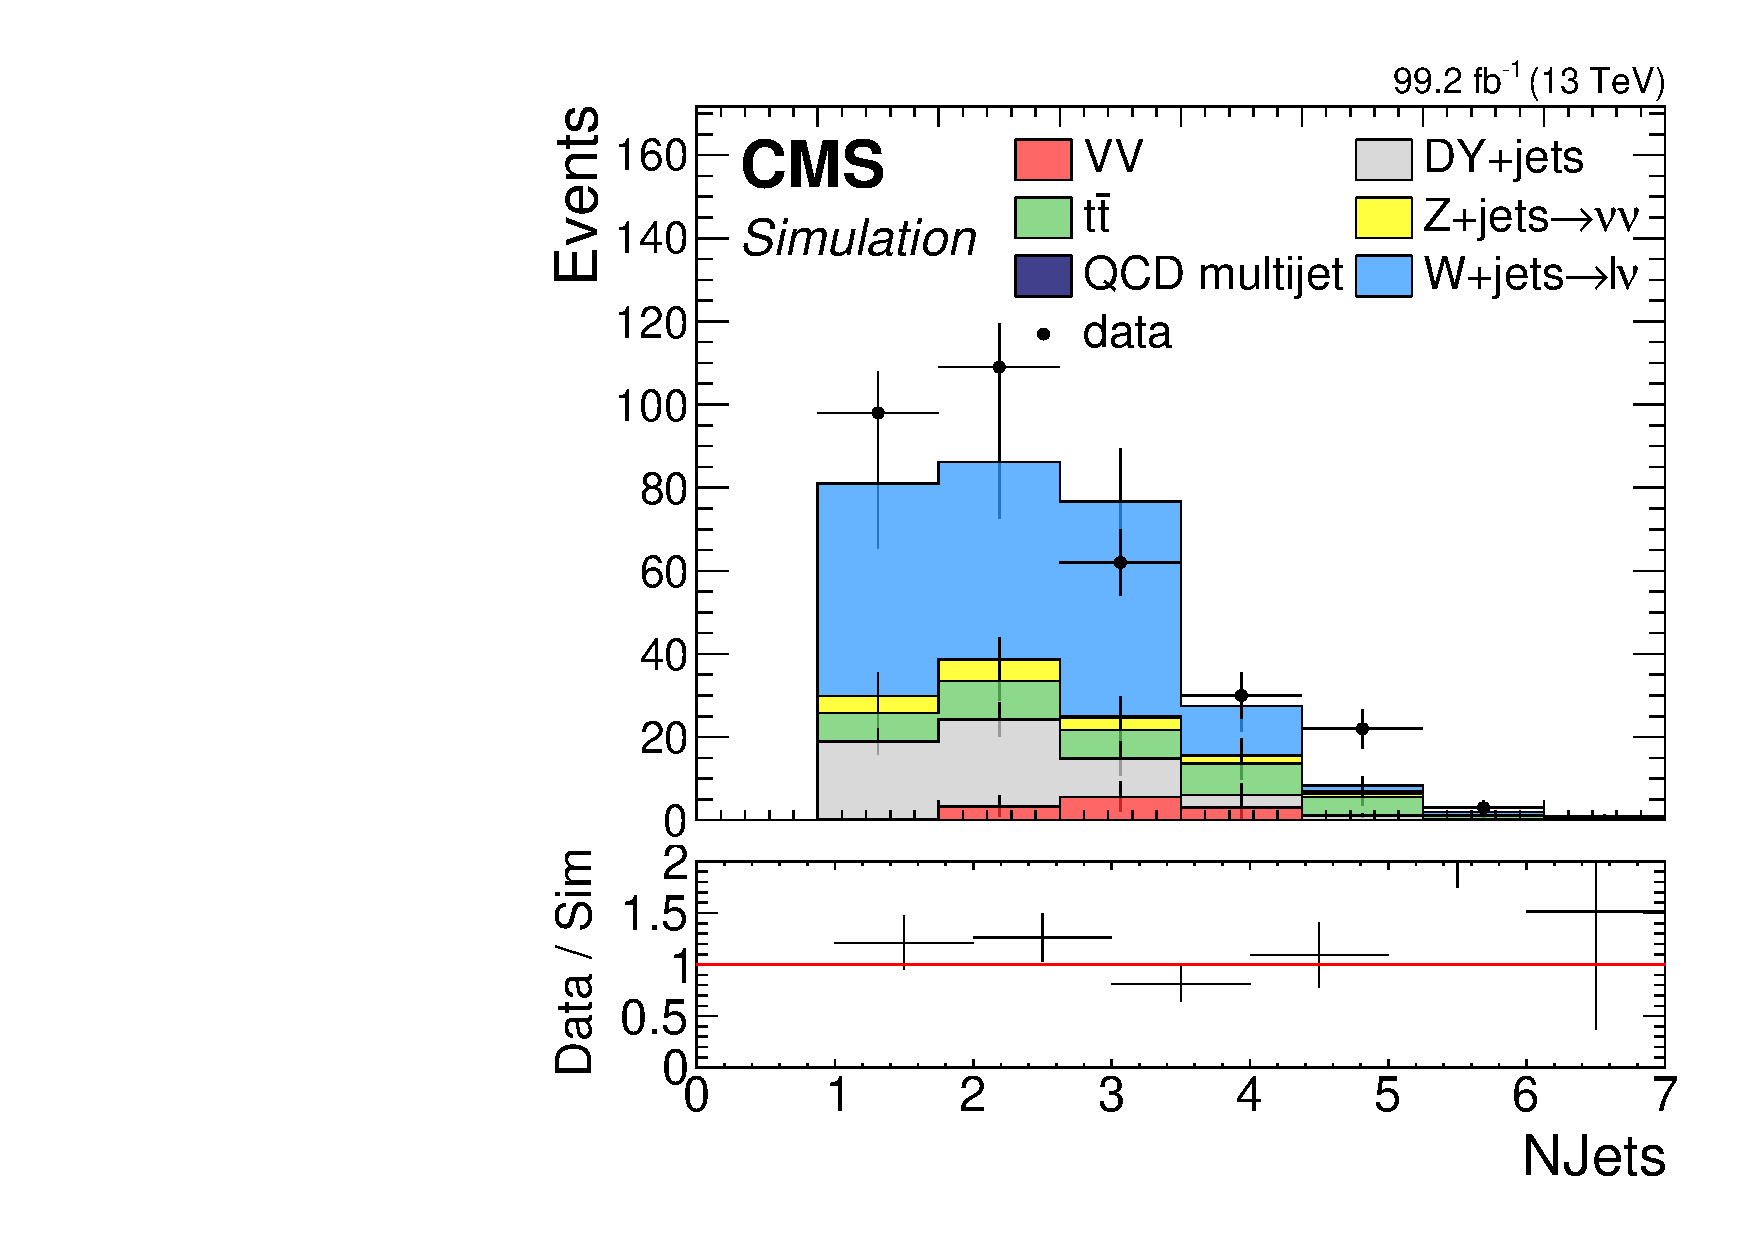
\includegraphics[width=0.48\linewidth]{plots/dilepton_muons_data_control_region_phase1/none_NJets.pdf} \\

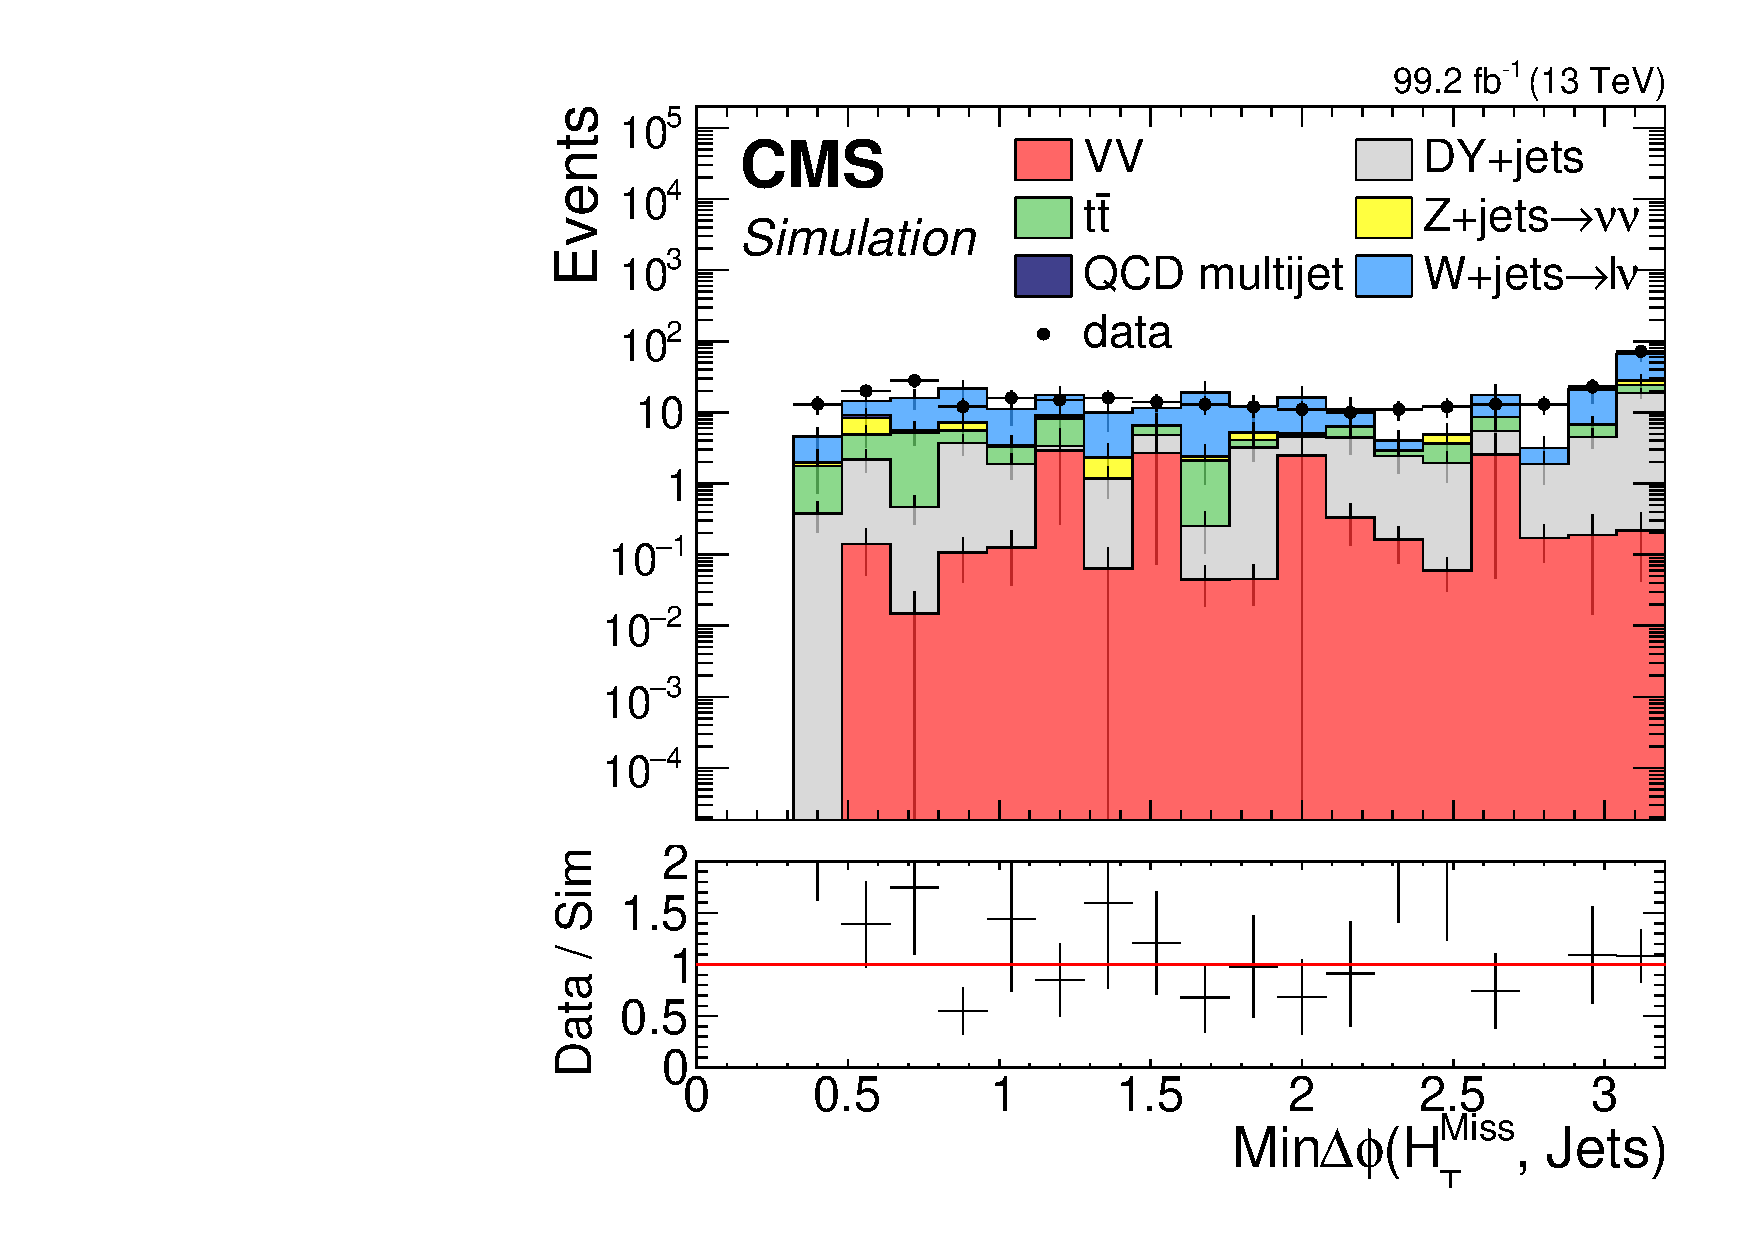
\includegraphics[width=0.48\linewidth]{plots/dilepton_muons_data_control_region_phase1/none_MinDeltaPhiMhtJets_log.pdf} \,
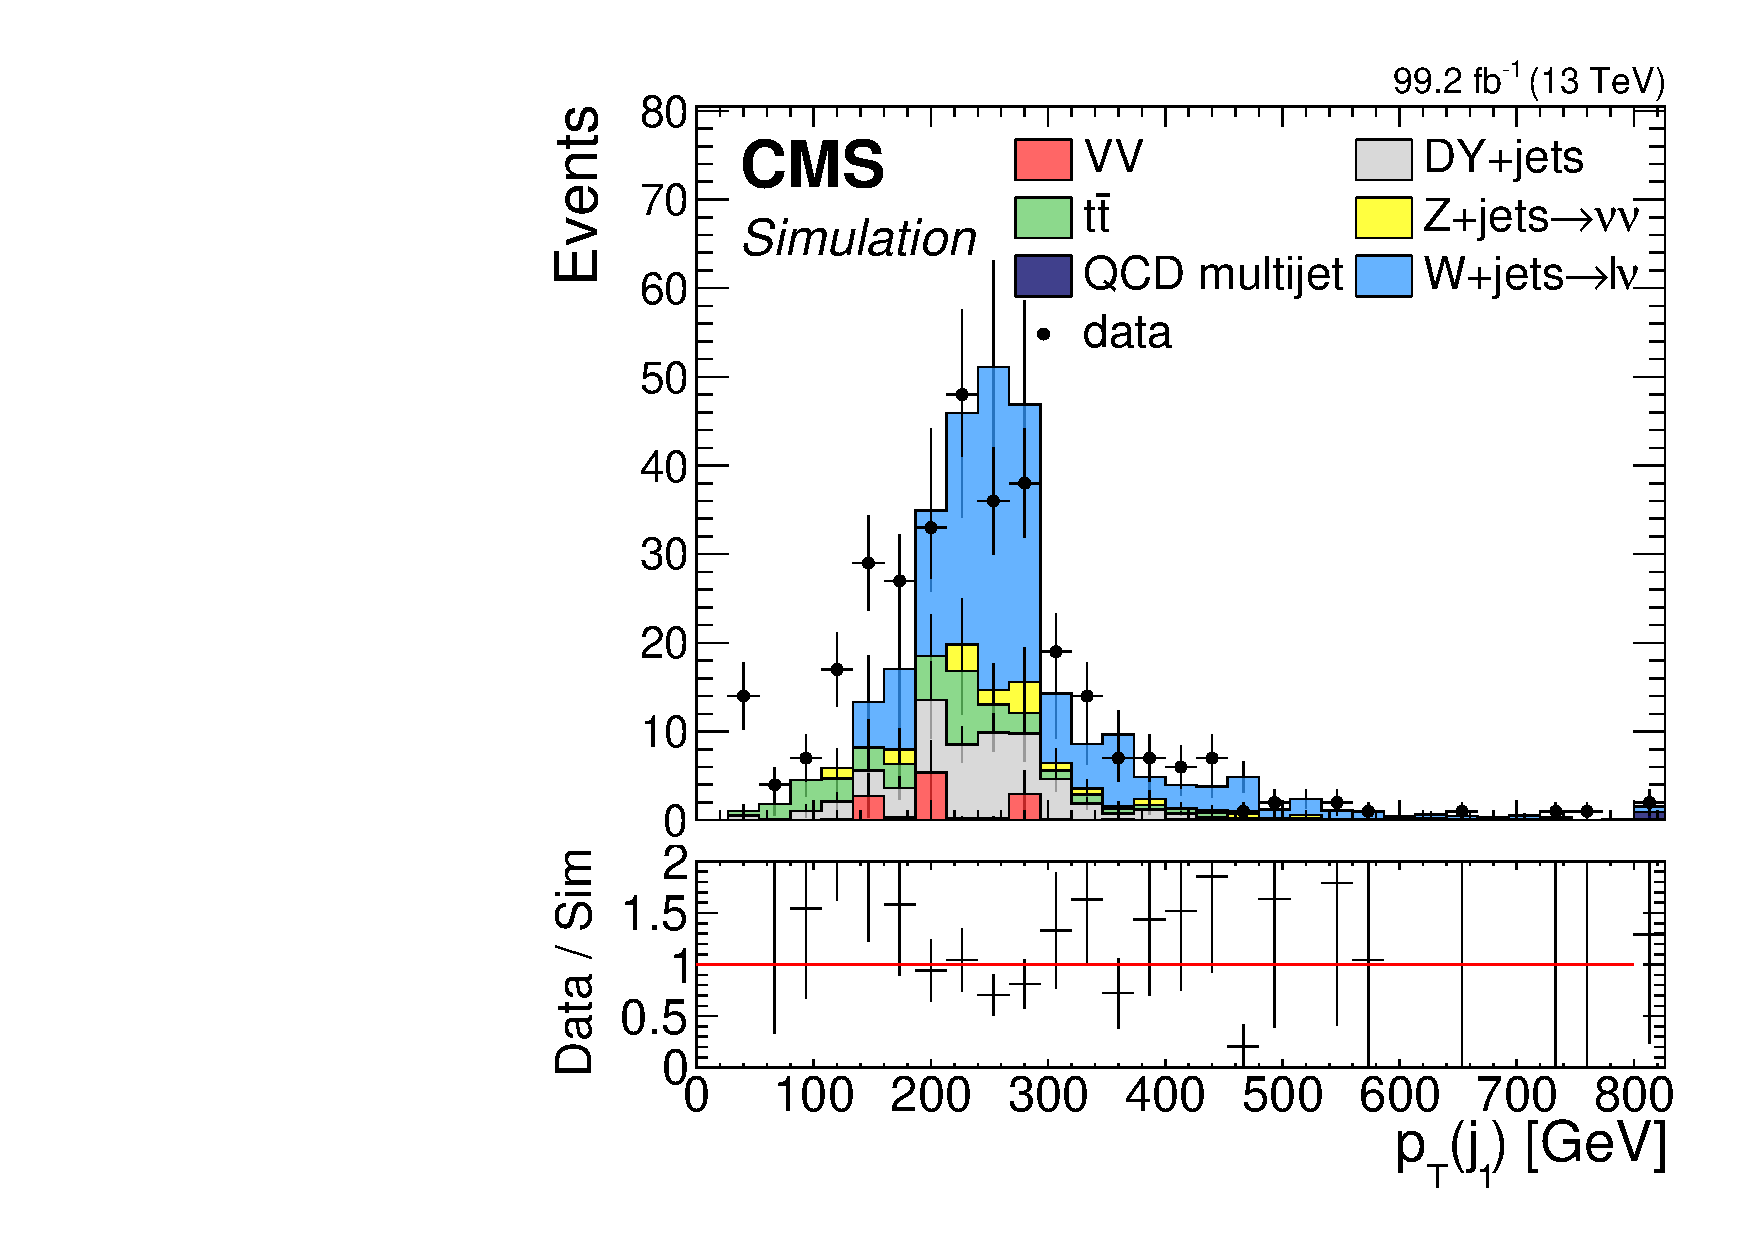
\includegraphics[width=0.48\linewidth]{plots/dilepton_muons_data_control_region_phase1/none_LeadingJetPt.pdf} \\

\caption[Data control region plots for dimuon category in phase 1]{Data control region plots for dimuon category in phase 1.}
\label{fig:data-control-plots-dimuon-phase1}
\end{figure} 


\begin{figure}[!htb]
\centering
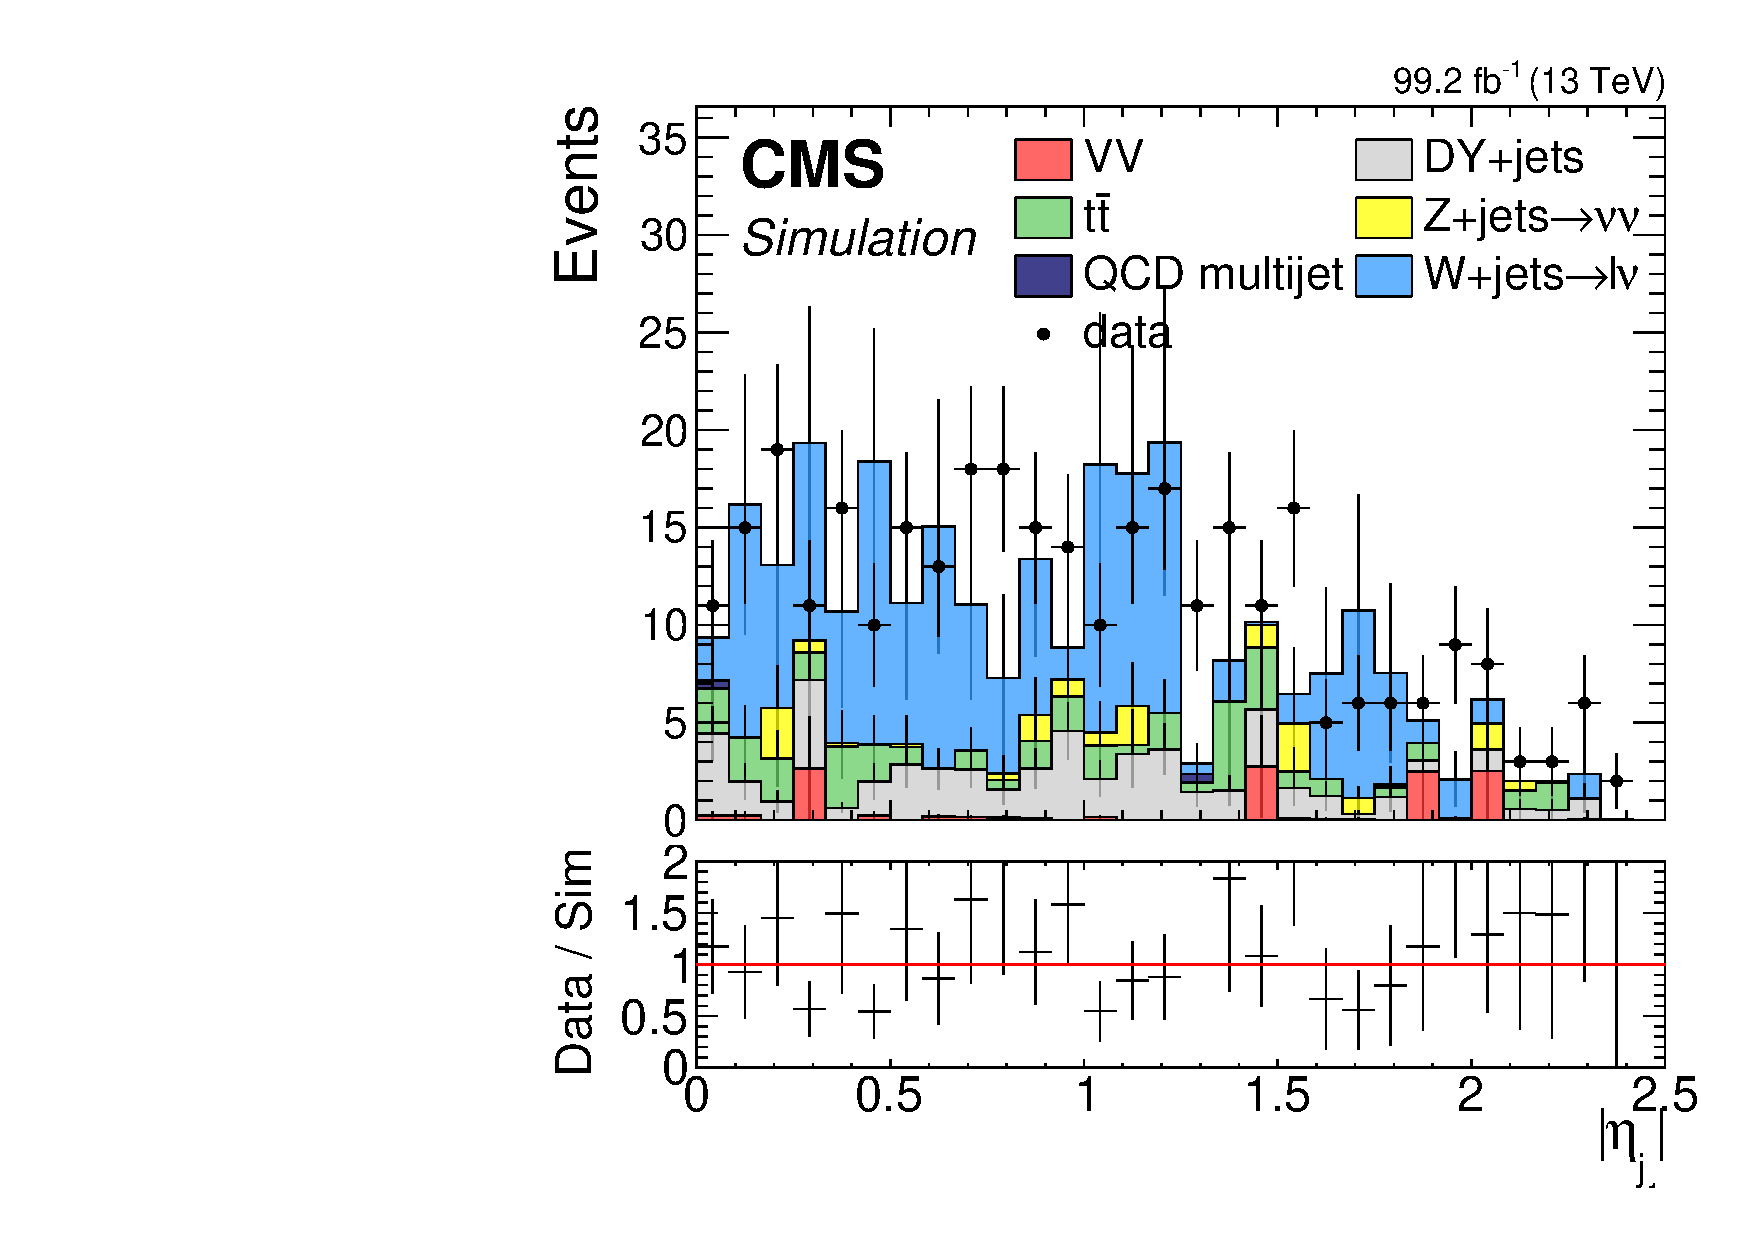
\includegraphics[width=0.48\linewidth]{plots/dilepton_muons_data_control_region_phase1/none_abs(LeadingJet.Eta()).pdf} \,
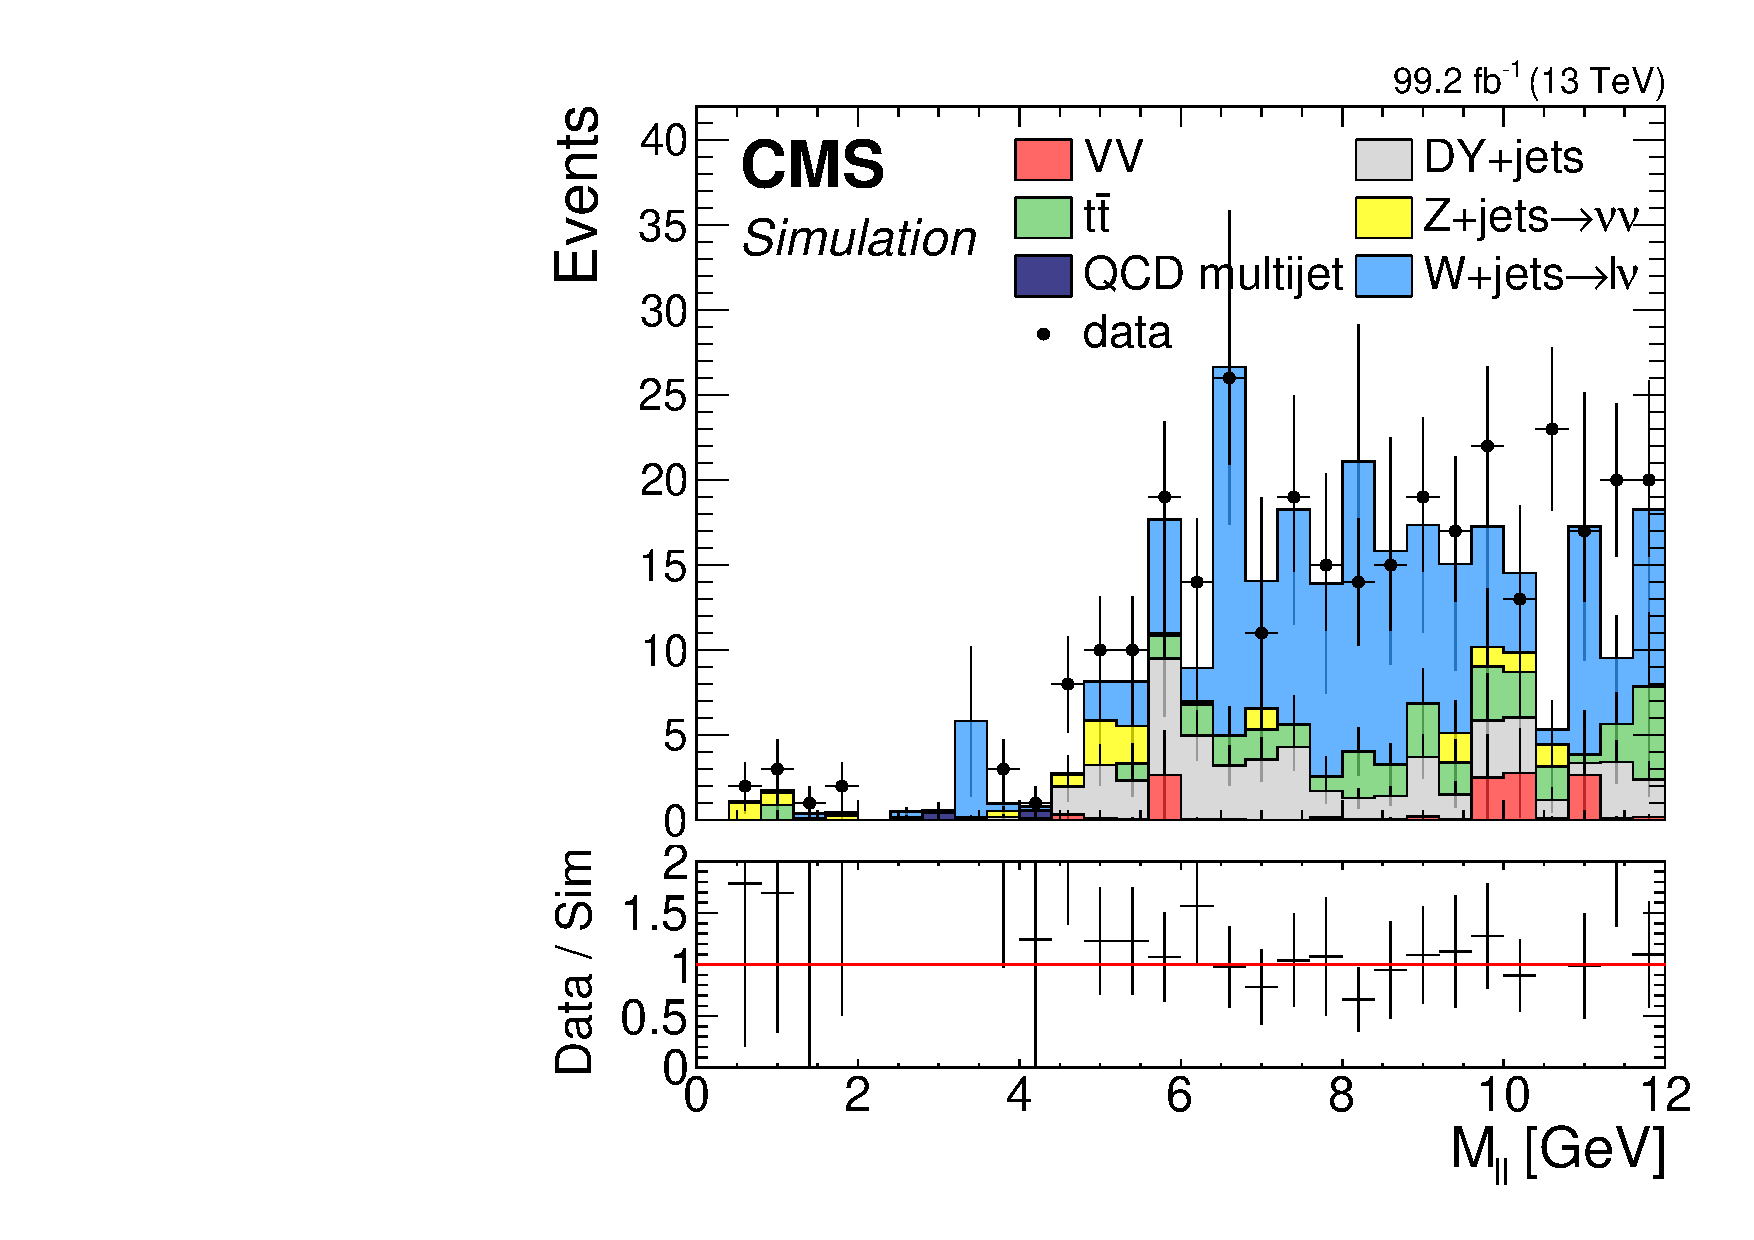
\includegraphics[width=0.48\linewidth]{plots/dilepton_muons_data_control_region_phase1/none_invMassCorrJetNoMultIso10Dr0.6.pdf} \\

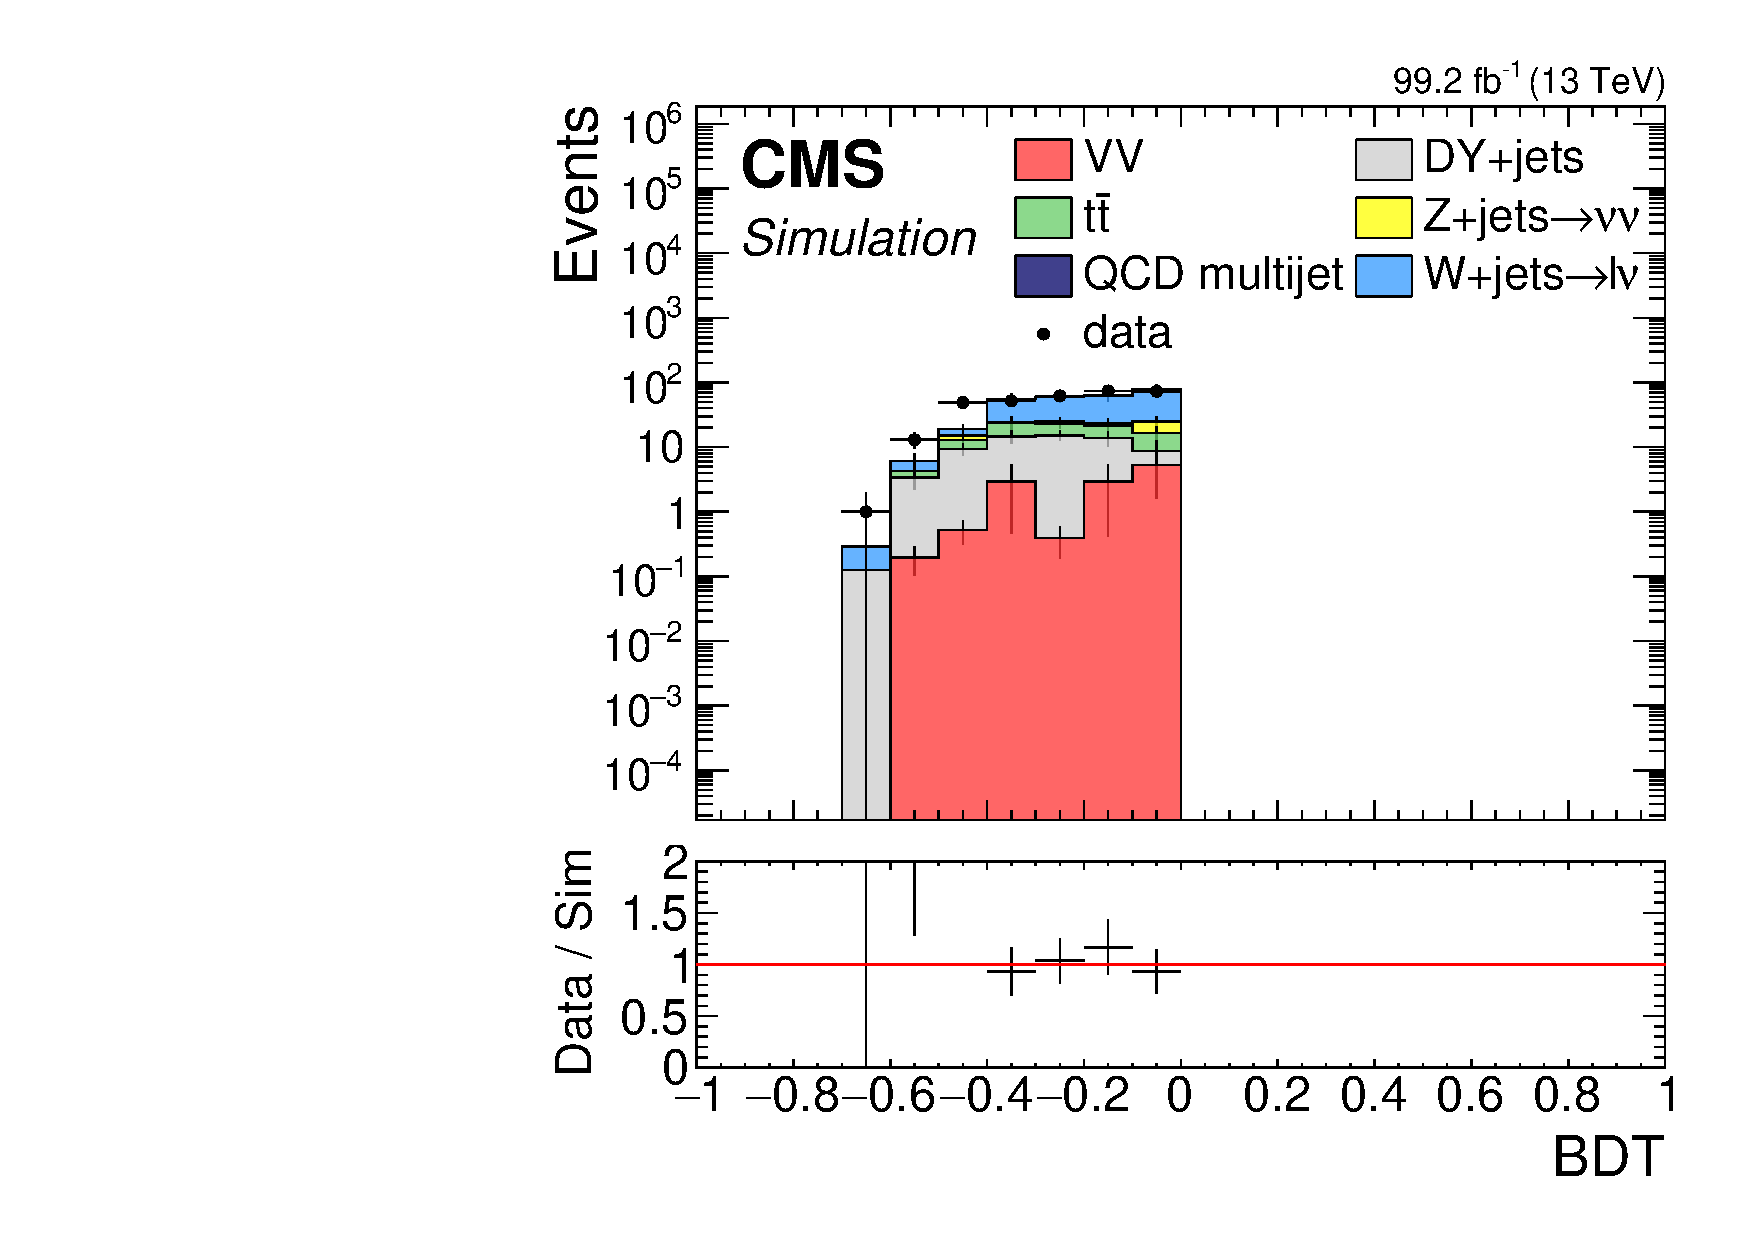
\includegraphics[width=0.48\linewidth]{plots/dilepton_muons_data_control_region_phase1/none_custom_dilepBDTCorrJetNoMultIso10Dr0.6_log.pdf} \,
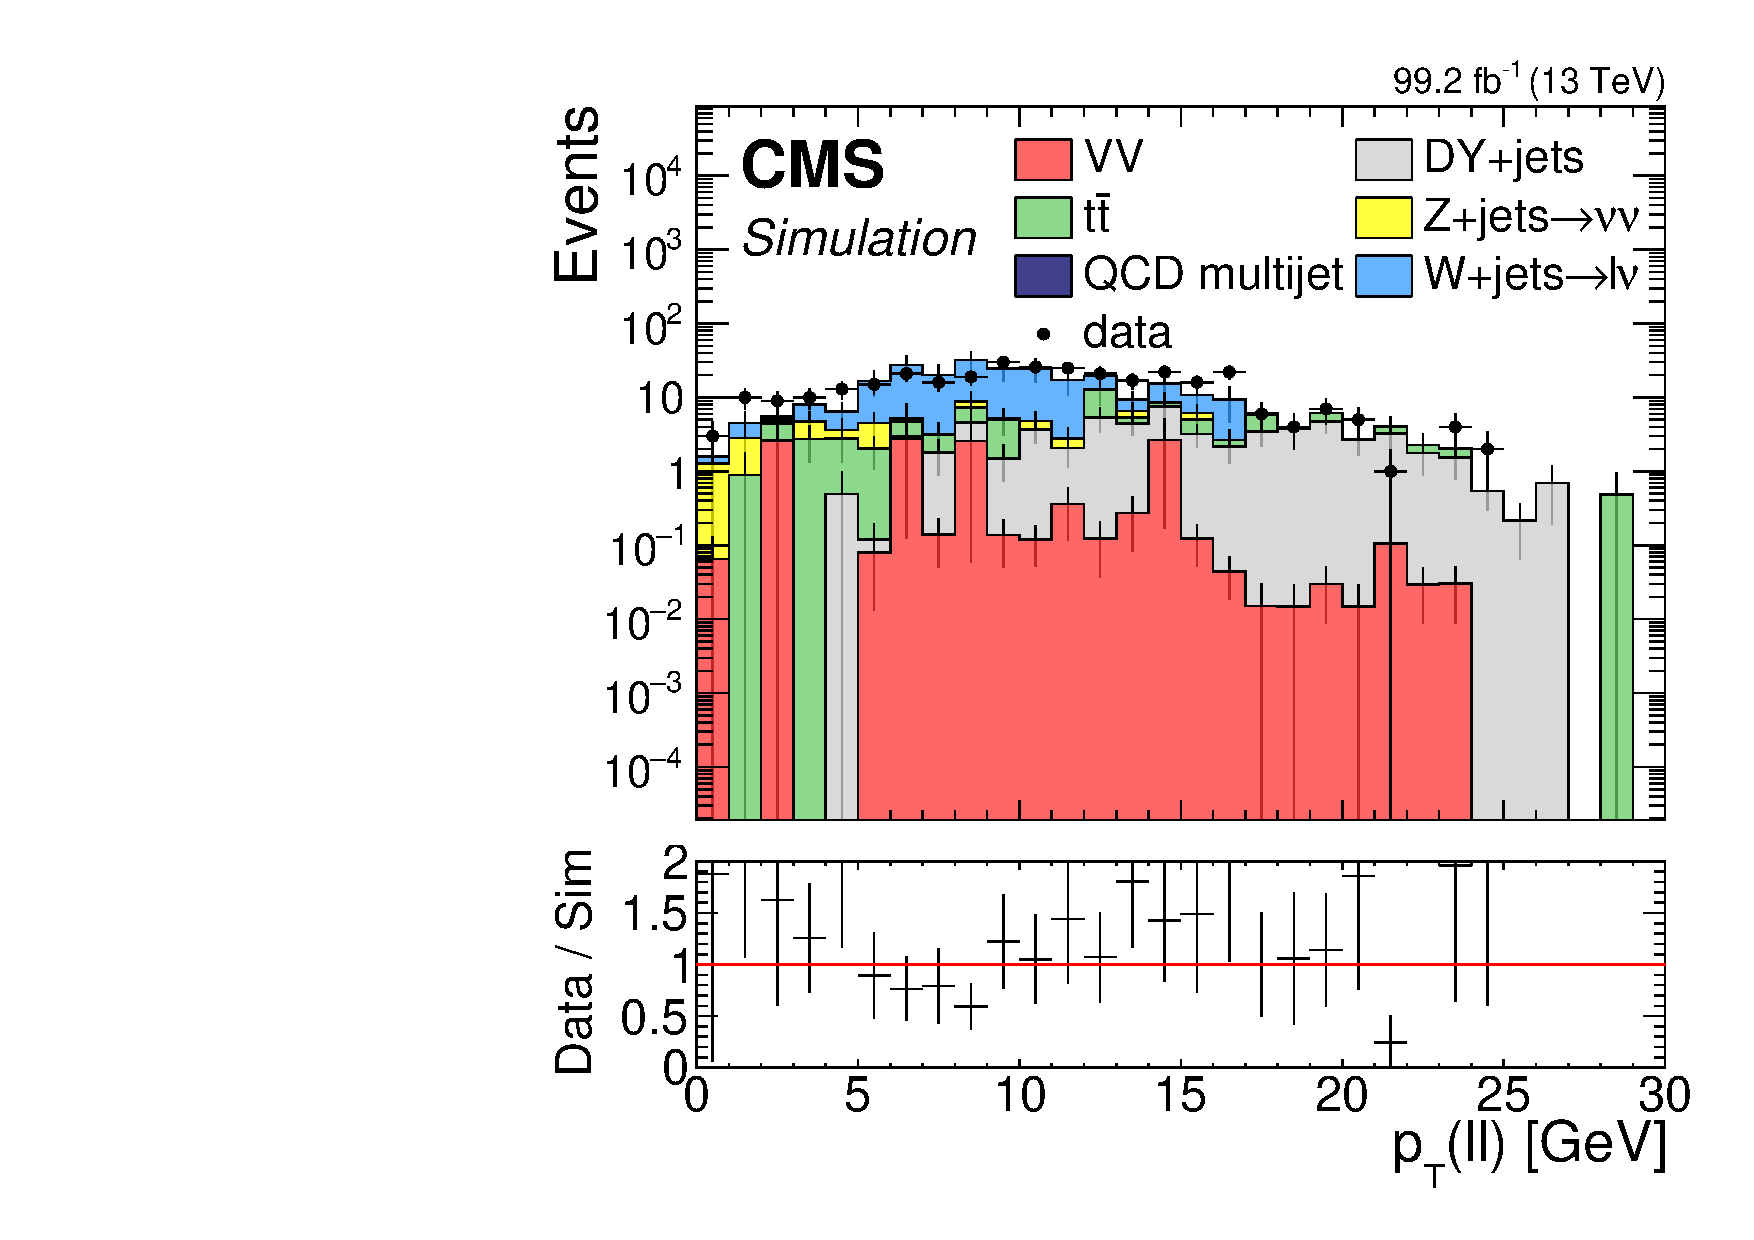
\includegraphics[width=0.48\linewidth]{plots/dilepton_muons_data_control_region_phase1/none_dileptonPtCorrJetNoMultIso10Dr0.6_log.pdf} \\

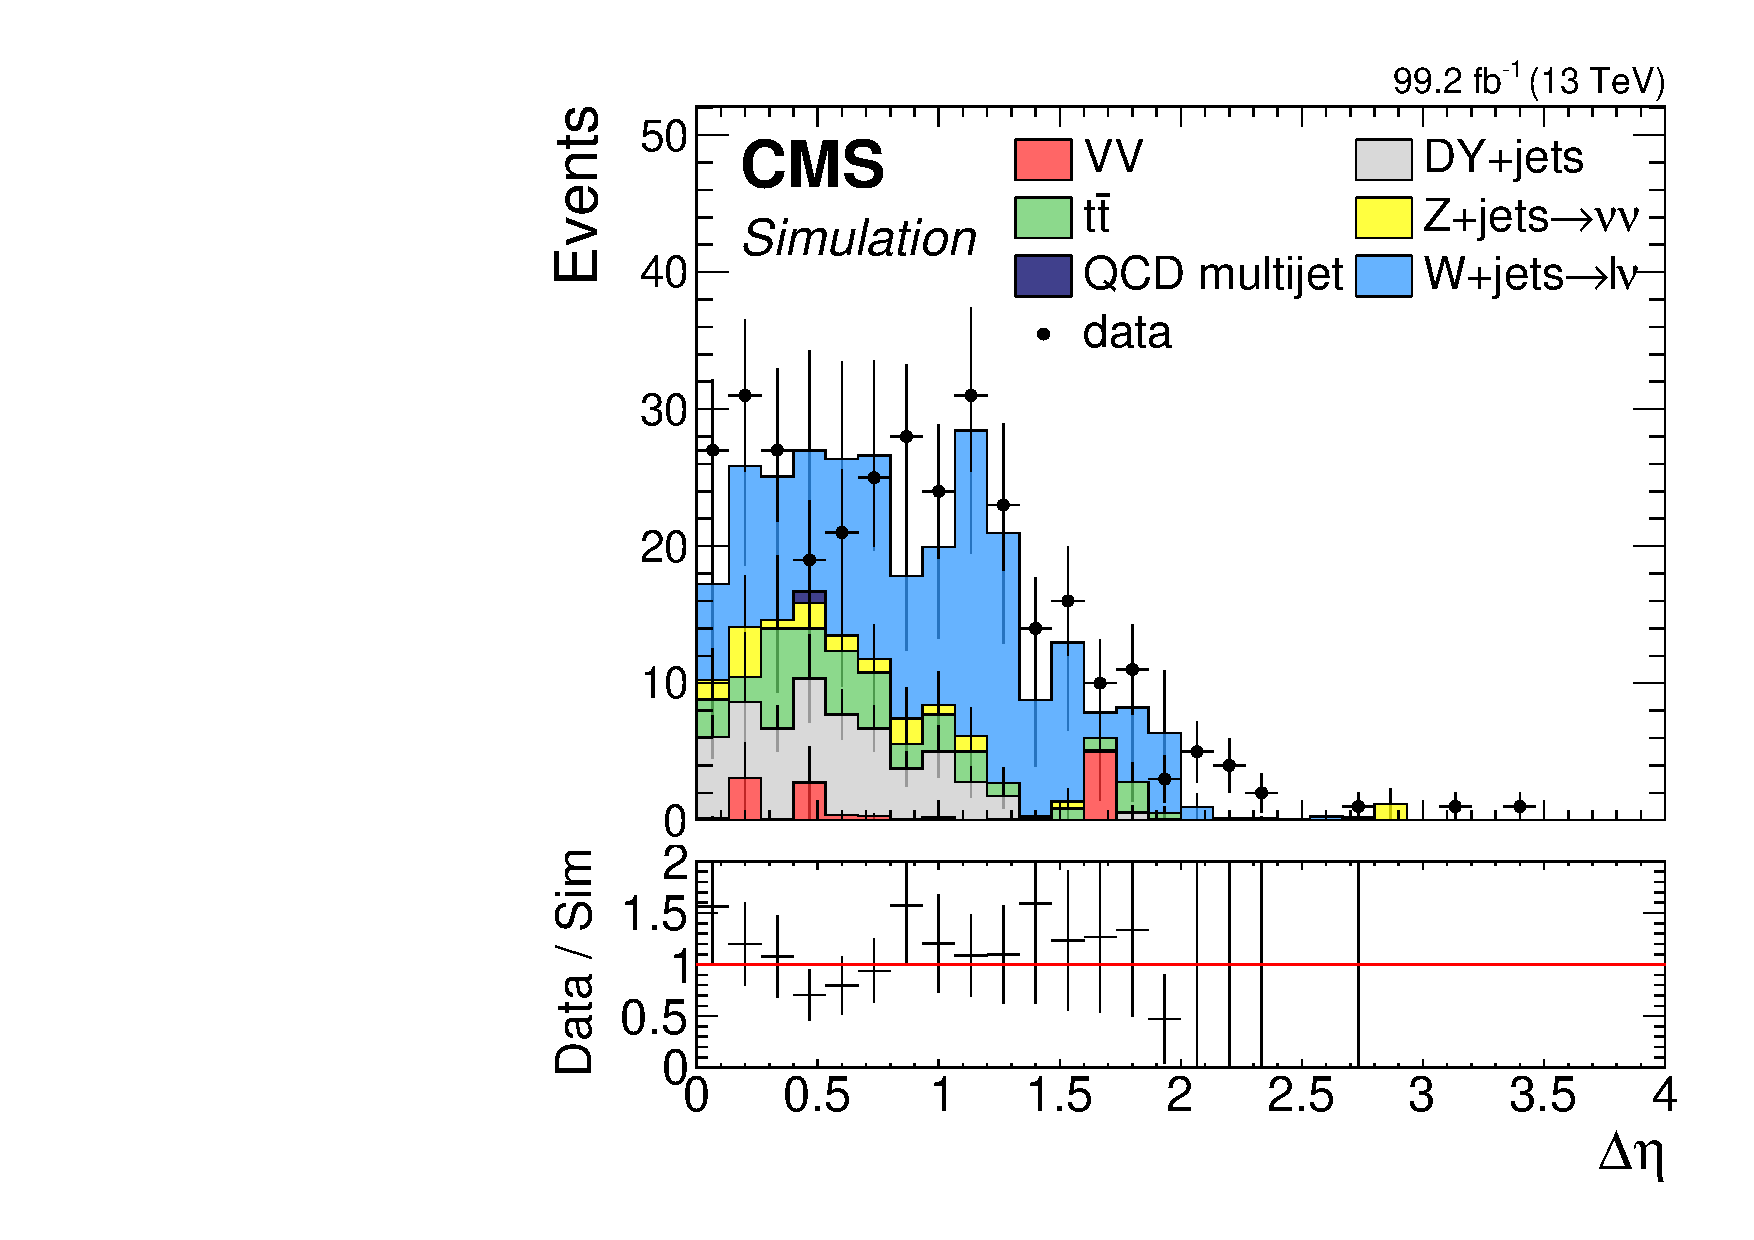
\includegraphics[width=0.48\linewidth]{plots/dilepton_muons_data_control_region_phase1/none_deltaEtaCorrJetNoMultIso10Dr0.6.pdf} \,
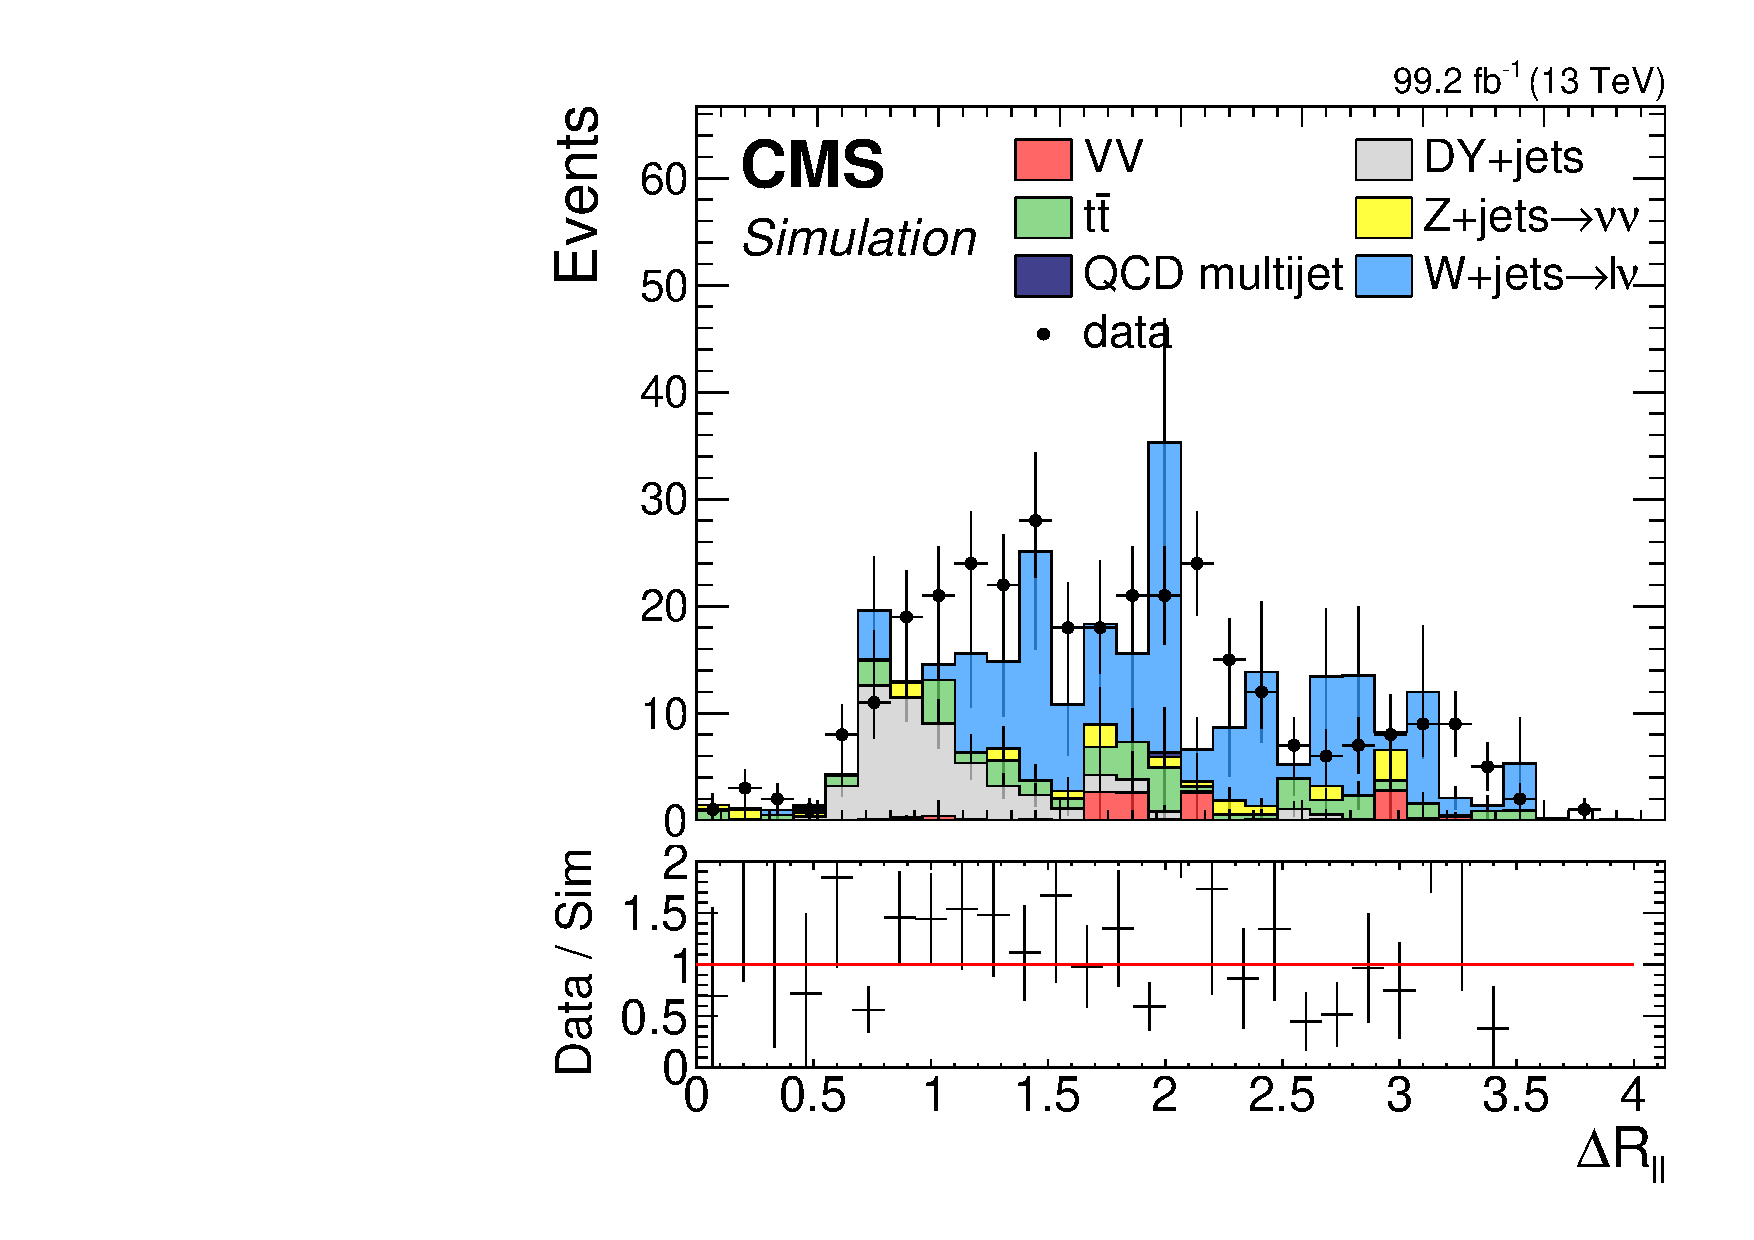
\includegraphics[width=0.48\linewidth]{plots/dilepton_muons_data_control_region_phase1/none_deltaRCorrJetNoMultIso10Dr0.6.pdf} \\

\end{figure} 